Das Water Indikator Tape stammt ursprünglich aus der Qualitätssicherung im dem Elektronikbereich und wird beispielsweise in Handys verwendet, um das Eindringen von Wasser nach zu weisen. Wenn das Tape rot wird, ist Wasser eingedrungen und der Hersteller kann eine Garantieleistung ablehnen.

Sobald das papierbasierte Klebeband nass wird, blutet die rote Farbe auf der Unterseite des Klebebands irreversibel durch das weisse obere Papier hindurch.

 Varianten von Water Indikator Tapes wurden ebenfalls getestet. Für diese Arbeit wurde das Produkt 5559 des Herstellers 3M ausgewählt, da es sich durch seine dünnere Dicke und damit schnellere Anzeigegeschwindigkeit auszeichnet.

Bei der Patent-Recherche zur Messung des LWC im Schnee wurde keine Verwendung von Water Indikator Tapes festgestellt, was auf die Neuartigkeit der Methode hindeutet. Der Hinweis, dass das Water Indikator Tape für die Messung des LWC genutzt werden kann, kam von Herr Loichinger.

Um die Interaktion des flüssigen Wasser mit dem Tape besser zu verstehen, wurde die Hydrophilie des Tapes getestet. Dazu wurde ein Wassertropfen auf das Tape gesetzt und der Kontaktwinkel gemessen. Im Abbildung \ref{fig:winkTropf} ist zu sehen, dass der Winkel zwischen dem Wasser und dem Tape etwa 90 Grad beträgt, was bedeutet, dass das Tape sich an der Grenze zwischen hydrophob und hydrophil befindet.

\begin{figure}
    \centering
    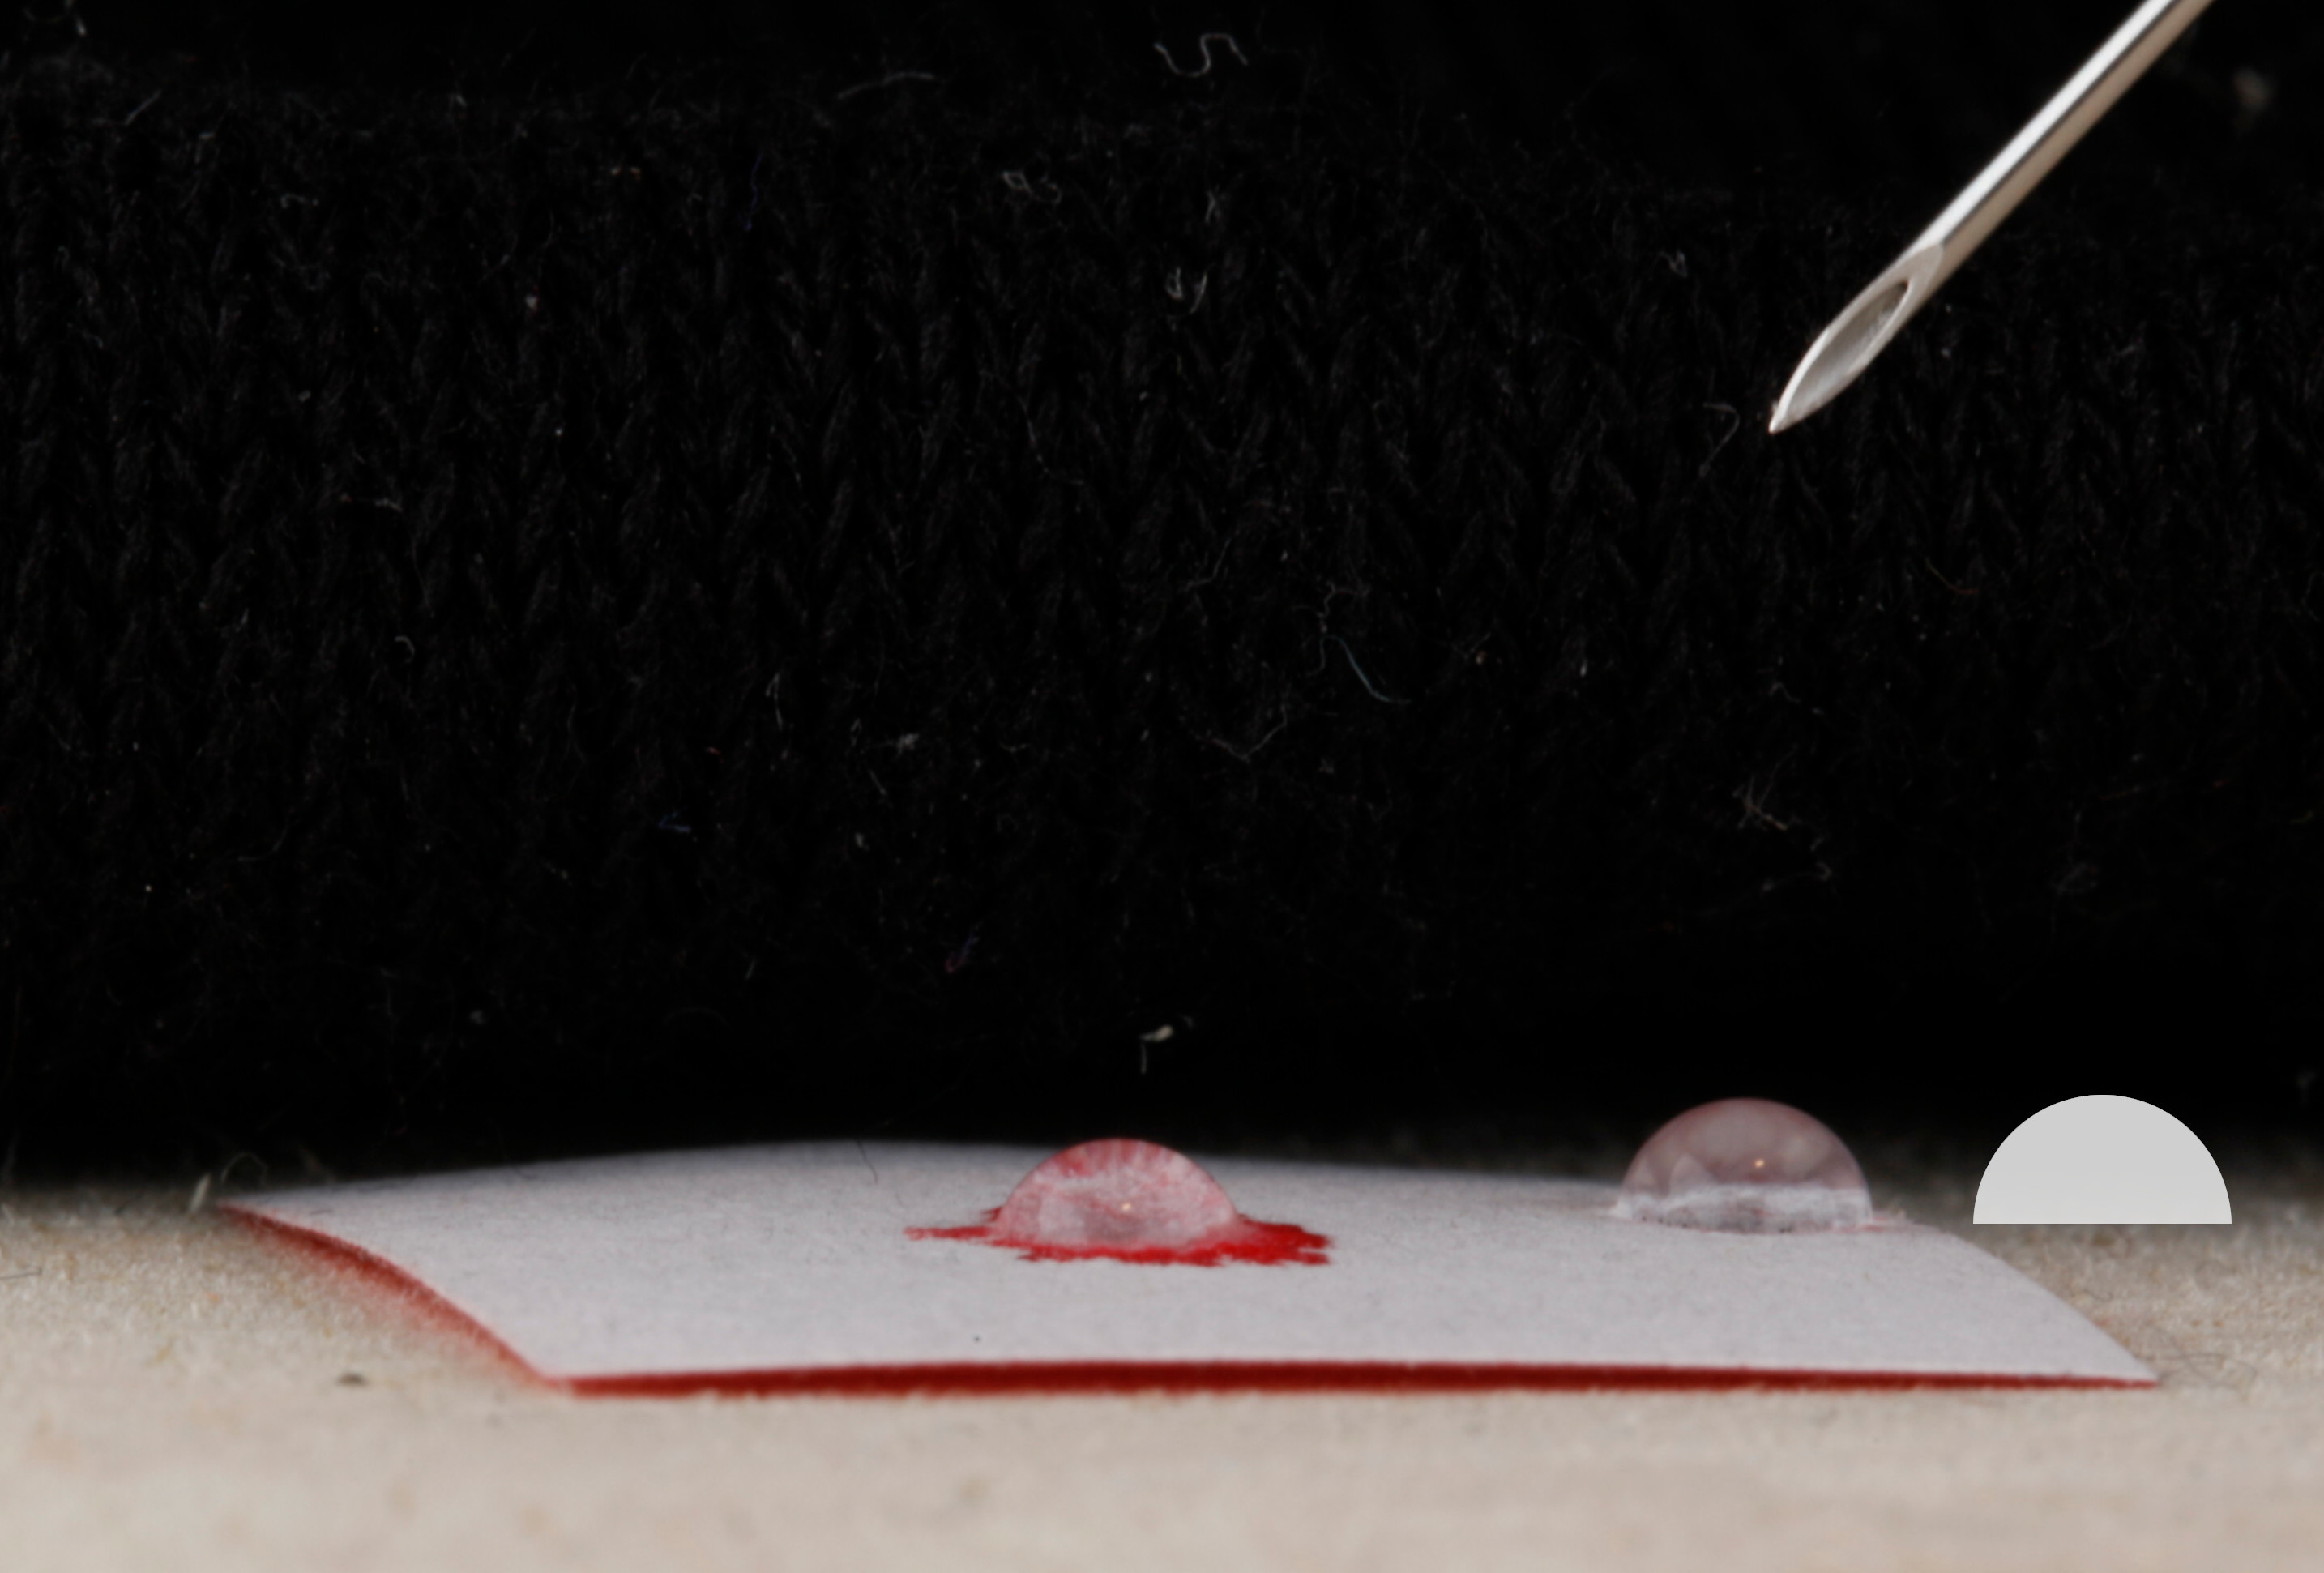
\includegraphics[width=0.8\textwidth]{Bilder/IMG_6683.JPG}
    \caption{Messung des Kontaktwinkels. Links ist ein Tropfen zu sehen, der mehrere Minuten auf dem Tape verweilt. Rechts ist ein neuer Wassertropfen, daneben noch der gefittete Kreis.} 
    \label{fig:winkTropf}
\end{figure}

Die Verfärbungen des Tapes sind abhängig von der Andruckdauer, Anpressdruck, der Geometrie des Schnees, dem Messablauf und dem LWC.

Bei einem ersten Feldversuch \ref{ersterFeldVer} konnten vielversprechende Ergebnisse gemessen werden.

\iffalse

Das 5559 Tape ist kostengünstig und zeigt innerhalb von weniger als 60 Sekunden das flüssige Wasser in einer Schicht an. Allerdings muss die Dichte des Schnees separat gemessen werden, da das Tape nur das flüssige Wasser anzeigt. Der Testaufbau beinhaltete das Kleben des 5559 Tapes auf ein rund 200 g schweres Objekt, das Freilegen einer neuen Schneeoberfläche mit einem Messer, das Auflegen des Tapes auf den Schnee und das Warten für 10, 30, 60 und 120 Sekunden. Anschließend wurde das Klebeband fotografiert und die rote gegen die weiße Fläche entweder optisch oder mithilfe von Python berechnet.

herkunft: Aus dem Elektronik bereich. zum beispiel in handys. wenn das tape rot geworden ist, ist wasser eingedrungen und der Hersteller kann eine garatieleistung ablehnen.

Funktionsweise: das papier basierte klebeband wird nass. die rote Farbe auf der Unterseite des Klebebands blutet durch das weisse obere Papier. die Roten Teile zeiget dann permanet wasser an.

Auswahl von 5559: der Hersteller 3M hat mehrere Produkte zu Water Indikator. 5559 zeichnet sich durch die dünnere Dicke und somit durch die schneller Anzeigegeschwindigkeit aus.

5559i ist auf einem transparenten substrat, was fraktisch für die optische auswertung wäre. Die Produkte sind in europa nur teilweise erhältlich. 3M verkauft nur Rollen mit 160 m. Zum testen wurde eine kleine rolle von einem Elektronikkomponenten Vertreiber gekauft.

Bei der Recherche zu LWC wurde keine verwendung von Water indicator tapes bemerkt. somit neuartig.

kostengünstig

zeitspanne pro messung weniger als 60 sek.

Dichte des Schnees muss seperat gemessen werden. 5559 zeigt nur das flüssige wasser in einer schicht an.

Testaufbau: 5559 auf etwas rund 200 g schweres kleben. neue Oberfläche von schnee mit Messer abschneiden/freilegen. 5559 auf schnee legen und 10, 30 60, 120 sek warten. foto von klebeband machen. mit python rote vs. weise fläche berechnen. oder nur optisch beurteilen.
\fi
